\documentclass[../main.tex]{subfiles}

\newcommand{\cI}{\mathcal{I}}
\begin{document}

\section{Backreaction and quantum corrections}
\label{sec:br}

We proceed to compute one-loop corrections to the OPE including those arising from the presence of the backreaction. This will complete the determination of the planar OPEs of the chiral algebra. To compute non-planar corrections, one would need to repeat this procedure for a larger class of bulk diagrams including 1. diagrams with loops in the bulk incorporating KS interactions, and 2. diagrams with $\leq 2$ backreaction legs attached to the defect plus an arbitrary number of bulk-defect propagators. The holomorphic integrals quickly get difficult when working beyond the box topology, but we remark that a class of non-planar contributions to the OPE of two open-string bulk operators (that is, considering additional space-filling D-branes coupled to KS theory), has been computed in \cite{} using homotopy transfer. These corrections, valid for a chiral algebra dual to Kodaira-Spencer plus space-fillng D-branes theory on the conifold, can be appended immediately to our chiral algebra, but does not yet include any dependence on the fermionic variables of the internal compactification manifold. One can view the non-planar contributions of \cite{} as incorporating diagrams of the second type (i.e. those without KS bulk loops). It would be very interesting to understand if other techniques from homological algebra can be leveraged to more directly obtain other non-planar contributions. 

We now turn to completing our study of the planar chiral algebra.

In this section we will use the following notations.

The holomorphic coordinate on $\C^3$ will be $Z = (z , w)$ where $w = (w^1,w^2)$ is a holomorphic coordinate on $\C^2$.
The defect will be located along $w = 0$.
In the formulas below, our convention is that $Z^0 = z$ and $Z^i = w^i$ for $i=1,2$.

\subsection{Warmup: holomorphic Chern--Simons theory}

Consider holomorphic Chern--Simons in the presence of a Kodaira--Spencer field which sources a brane wrapping $N$ $D1$ branes $\C \subset \C^3$. 
The backreaction field is 
\[
\mu_{BR} = N \frac{\eps_{ij} \wbar^i \d \wbar^j}{4 \pi^2 \|w\|^4} \partial_z \in \PV^{1,1} (\C^3 \setminus \C) . 
\]
This field satisfies the equation
\beqn\label{eqn:csBR}
\dbar \mu_{BR} \wedge \Omega_{w_i=0} = N \delta_{w_i = 0} \del_z 
\eeqn
where $\delta_{w_i=0}$ is the $\delta$-function supported at $w_i=0$.
This couples to the holomorphic Chern--Simons field by 
\[
S_{BR} = \frac12 \int_{\C^3} \mu_{BR} \vee \op{tr}(A \del A) = \frac12 N \int_{\C^3} A^a \frac{\eps_{ij} \wbar^i \d \wbar^j}{\|w\|^4} \partial_z A^a .
\]
We will denote $\omega = \frac{\eps_{ij} \wbar^i \d \wbar^j}{4 \pi^2\|w\|^4}$ so that the coupling can be written $S_{BR} = \frac{N}{2}
\int_{\C^3} A \omega \del_z A.$

The backreaction coupling has a gauge anomaly even at tree-level.
Indeed, the tree-level gauge variation of $S_{BR}$ is
\[
\int_{\C^3} A^a (\dbar \mu_{BR}) \fc^a = \int_{\C_z} A_{\zbar}^a \partial_z \fc^a .
\]
In order to cancel this gauge anomaly one must introduce an $N$-dependent term in the OPE of the currents $J_a[k,l]$. 
In fact, at tree level only the OPE between currents with $k=l=0$ 
is affected by the tree-level backreaction.
In the presence of the backreaction the currents $J_a[0,0]$ form a Kac--Moody algebra of level $N$
\[
J_a[0,0] (0) J_b [0,0] (z) \simeq f_{ab}^c \frac1z J_c[0,0] + \delta_{ab} N \frac1{z^2} {\rm Id} .
\]
The second term in the OPE is present due the the existence of a tree-level anomaly which involves the back reaction.
The diagram which represents this anomaly is given in figure \ref{fig:treeBR}.

What about higher loop anomalies involving the backreaction?
For scaling dimension reasons, there are no further corrections to the $J_a[0,0]-J_b[0,0]$ OPE.
Let's consider the possibility of quantum corrections to the OPE between the fields $J_a[1,0]$ and $J_b[0,1]$. 
Before accounting for the back reaction, the tree and one-loop level OPE is 
\beqn\label{eqn:Jbr}
J_a[1,0](z) J[0,1]_b \simeq \frac{1}{z} f^c_{ab} J[1,1] + \hbar \frac1z K^{fe} f_{ae}^c f_{bf}^d J_c[0,0] J_d[0,0] ,
\eeqn
see section ?? of \cite{CPkoszul}.
By conformal invariance, the possible $N$-dependent terms in the OPE $J_a[1,0] (0) J_b [0,1](z)$ must be of the form
\[
\alpha f^c_{ae} K^{be}  \left(\frac{1}{z^2} J_c[0,0] + \frac{1}{z} \del_z J_c[0,0] \right) + \beta K^{ab} \frac{1}{z^3} {\rm Id} 
\]
for some (possibly zero) constants $\alpha,\beta$ which depend on~$N$
(notice that the form of the central term in the last term is consistent with the fact that $J[1,0], J[0,1]$ are of spin $3/2$).
The diagrams which give rise to the anomalies necessitating these terms in the OPE are given in figures \ref{fig:loopBR1} and \ref{fig:loopBR2}, respectively.
In these diagrams, the dotted lines represent coupling to the backreaction and the wiggle lines represent bulk propagators.

As usual, to evaluate these diagrams we use point splitting on the defect so that operators are placed at $z_1$,$z_2 \in \C$ with $|z_1-z_2| \geq \epsilon$.
In appendix \ref{appx:hcsbr} we show by direct computation that the weight of the one-loop diagram in figure \ref{fig:loopBR2} is
\beqn
N^2 K_{ab} \eps_{ij} \int_{|z_1-z_2| \geq \epsilon} \frac{1}{(z_1 - z_2)^3} \del_{w_i} A^a_1 \del_{w_j} A^b_2 |_{w=0},
\eeqn
where $A_1,A_2$ are the input gauge fields.
The linear BRST variation $A \mapsto A + \dbar c$ of this diagram thus gives rise to the anomaly
\beqn
N^2 K_{ab} \eps_{ij} \int_{|z_1-z_2| \geq \epsilon} \frac{1}{(z_1-z_2)^3} \del_{w_1} A^a \del_{w_2} \dbar c^b |_{w=0}
\eeqn
Integrating by parts and taking $\epsilon \to 0$ this anomaly becomes
\beqn
N^2 K_{ab} \eps_{ij} \del^3 \delta_{z_1=z_2} \del_{w_1} A^a \del_{w_2} \dbar c^b |_{w=0} .
\eeqn
In this form it is clear that this anomaly is canceled by introducing the term in the OPE in \eqref{eqn:Jbr} with
\beqn
\beta = ?? .
\eeqn
\brian{just need to work out the constants}

\begin{figure}
	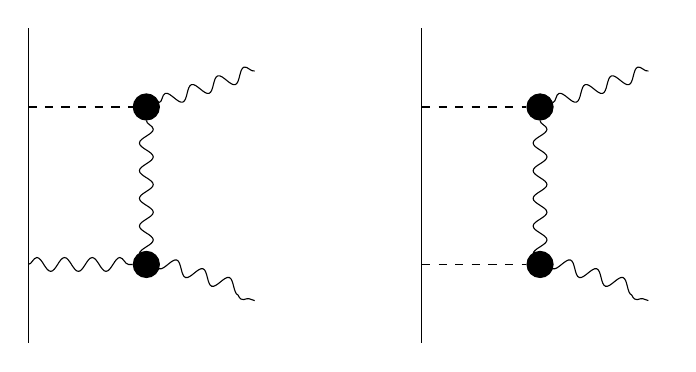
\begin{tikzpicture}
	\begin{scope}		
			\node (A1) at (3,1.5) {};
			\node (A2) at (3,-1.5){};

		\node[circle,draw,fill=black]  (V1) at (1.5,1) {}; 
		\node[circle,draw,fill=black]  (V2) at (1.5,-1) {};  
		\draw[decorate, decoration={snake}]  (V1) --  (A1);
		\draw[decorate, decoration={snake}] (V1) -- (V2) -- (A2);
		\draw[decorate,decoration={snake}](0,-1) -- (V2);
		\draw[dashed] (0,1) -- (V1);

		\draw (0,2) -- (0,-2);	
	\end{scope}

		\begin{scope}[shift={(5,0)}]		
			\node (A1) at (3,1.5) {};
			\node (A2) at (3,-1.5){};

		\node[circle,draw,fill=black]  (V1) at (1.5,1) {}; 
		\node[circle,draw,fill=black]  (V2) at (1.5,-1) {};  
		\draw[decorate, decoration={snake}]  (V1) --  (A1);
		\draw[decorate, decoration={snake}] (V1) -- (V2) -- (A2);
		\draw[dashed](0,-1) -- (V2);
		\draw[dashed] (0,1) -- (V1);

		\draw (0,2) -- (0,-2);	
	\end{scope}
	\end{tikzpicture}
	\label{fig:hcsback}
	\caption{Diagrams contributing to the first-order gauge anomaly in the presence of the backreaction in holomorphic Chern--Simons theory.}  
\end{figure}

\subsection{Tree-level backreaction in Kodaira--Spencer theory}

We now turn to our version of Kodaira--Spencer theory obtained by compactifying the twist of type IIB supergravity on a $K3$ surface.
The first nontrivial contribution from the backreaction occurs at tree-level. 
Part of this contribution was computed in \cite{CP}.
The backreaction field $\mu_{BR} = \mu_{BR}(\eta)$ takes a similar form as in the previous section.
It is a distributional section
\beqn
\mu_{BR} \in \PV^{1,1}(\C^3) \otimes A
\eeqn
which satisfies the defining distributional equation
\beqn
\dbar \mu_{BR} = \delta_{w_i=0} F^{ab} \eta_a \eta_b \del_z  .
\eeqn
The field $\mu_{BR}$ couples to the fields $\mu_i$ through
\beqn\label{eqn:brmu1mu2}
\int_{\C^3} \mu_{BR} \mu_1  \mu_2 |_{\eta \br \eta} \, \d^3 Z . 
\eeqn
It couples to the fields $\alpha ,\gamma$ through
\beqn\label{eqn:brag}
\int_{\C^{3}} \mu_{BR} \alpha \del_z \gamma |_{\eta \br \eta} \, \d^3 Z .
\eeqn
Notice that by type reasons the backreaction field does not couple to the Beltrami field~$\mu_z$ in the $\del_z$ direction.

Let's first consider the coupling \eqref{eqn:brmu1mu2}. 
The tree-level gauge variation of the backreaction coupling \eqref{eqn:brmu1mu2} as
\beqn\label{eqn:treeanomaly1}
\int_{\C^3} \mu_{BR} \dbar \lie{c}_1  \mu_2 |_{\eta \br \eta} \, \d^3 Z +  \int_{\C^3} \mu_{BR}  \mu_1  \dbar \lie{c}_2 |_{\eta \br \eta} \, \d^3 Z = \int_{\C} \left(\lie{c}_1 \mu_2 + \mu_1 \lie{c}_2\right)|_{\eta \br \eta, w = 0} .
\eeqn
Similarly, the tree-level gauge variation of the coupling \eqref{eqn:brag} is 
\beqn\label{eqn:treeanomaly2}
\int_{\C^3} \mu_{BR} \dbar \lie{c}_\alpha  \del_z\gamma |_{\eta \br \eta} \, \d^3 Z +  \int_{\C^3} \mu_{BR}  \alpha  \dbar \del_z\lie{c}_\gamma |_{\eta \br \eta} \, \d^3 Z = \int_{\C} \left(\lie{c}_\alpha \del_z \gamma + \alpha \del_z\lie{c}_\gamma\right)|_{\eta \br \eta, w = 0} .
\eeqn

Notice that neither of these expression involve $w_i$-derivatives. 
Since $\til{J}^i[0,0]$ couples to $\mu_i$, the anomaly in \eqref{eqn:treeanomaly1} can be cancelled by the gauge variation of 
\beqn
\int_{z,z'} \til{J}^1[0,0](z) \mu_1(z) \til{J}^2[0,0] (z') \mu_2(z')|_{\eta \br \eta \eta'\br\eta'} 
\eeqn
provided that the $\til{J}^i[0,0]$ operators satisfy an appropriate OPE. 
Similarly, the anomaly in \eqref{eqn:treeanomaly2} can be cancelled by the gauge variation of a coupling of the form
\beqn
\int_{z,z'} G_\alpha[0,0](z) \alpha(z) G_\gamma[0,0] (z') \gamma (z') |_{\eta \br \eta \eta'\br\eta'} 
\eeqn
(We are omitting appearences of volume forms for simplicity.)

Proceeding as above by working in the Fourier dual odd coordinates and working with on-shell fields, we see that to cancel the first of these anomalies there must be a term in the $\til J \til J$ OPE of the form
\beqn
\til{J}^i[0,0](0,\what\eta^a) \til{J}^j [0,0] (z,\what\eta'^a) \simeq \epsilon^{ij} \frac1z \what F (\what\eta^a + \what\eta'^a) .
\eeqn
Using the constraints \eqref{eqn:constraint1} we can write this OPE in terms of on-shell fields as
\beqn
J[1,0](0,\what \eta^a) J[0,1] (z,\what \eta'^a) \simeq \frac{1}{z} \what F(\what \eta^a + \what \eta'^a) .
\eeqn

Similarly, to cancel the second anomaly there must be a term in the GG OPE of the form
\beqn
G_\alpha[0,0](0,\what \eta^a) G_\gamma[0,0](z,\what \eta'^b) \simeq \frac1{z^2} \what F (\what \eta^a + \what \eta'^a) .
\eeqn

As a simple consequence of this, we see that the operators 
\[
J[1,0](\what \eta), J[0,1](\what \eta),G_\alpha[0,0](\what \eta), G_\gamma[0,0](\what \eta)
\]
form a subalgebra of the full gravitational chiral algebra.
Recall that the spin of the operator $G_\alpha[0,0]$ is one.
If we choose a spin zero operator $G'_{\alpha}[0,0]$ such that $\del G_\alpha'[0,0]$ then we can obtain the same OPE as above if we declare that 
\beqn
G'_\alpha[0,0](0,\what \eta^a) G_\gamma[0,0](z,\what \eta'^b) \simeq \frac1{z} \what F (\what \eta^a + \what \eta'^a) .
\eeqn
The operators $J[1,0](\what \eta), J[0,1](\what \eta),G
'_\alpha[0,0](\what \eta), G_\gamma[0,0](\what \eta)$ form a familiar chiral algebra of free fields.
\brian{finish, say what the free theory is more explicitly, refer back to CDR.}

\subsection{The propagator for Kodaira--Spencer theory}

The following discussion is based off the work \cite{CLbcov1}. 
We recall only the essential details. 

The propagator for Kodaira--Spencer theory on $\C^3$ is the kernel for the operator $\del \dbar^* \tr^{-1}$. 
We obtain this by applying the divergence operator to the kernel for the operator $\dbar^* \tr^{-1}$ (this is the propagator used in holomorphic Chern--Simons theory). 
Let us first recall the construction of the kernel for $\dbar^* \tr^{-1}$.

As usual, we use $(z,w_i)$ for a coordinate on $\C^3$. 
Using the Calabi--Yau form one can express the integral kernel for the operator $\dbar^* \tr^{-1}$ as
\[
P'(z,w_i) = \frac{1}{r^6} \big(\zbar \d \wbar_1 \d \wbar_2 - \wbar_1 \d \wbar_2 \d \zbar + \wbar_2 \d \zbar \d \wbar_1 \big) \del_z \del_{w_1} \del_{w_2}  
\]
where $r^2 = |z|^2 + |w_1|^2 + |w_2|^2$. 
This is a smooth section of $\PV^{3,2}(\C^3)$ away from $0 \in \C^3$.
The kernel is obtained by pulling back this section along the difference map 
\[
\C^3 \times \C^3 \to \C^3,\quad (z, w_i ; z',w_i') \mapsto (z-z', w_i - w_i') .
\]
We denote the pulled back section by
\[
P'(z,w_i ; z',w_i') \in \br{\PV}^{3,2}(\C^3 \times \C^3) . 
\]
Here $\br{\PV}^{3,2}$ stands for distributional Dolbeault valued polyvector fields of type $(3,2)$.
Notice that this section is smooth away from the diagonal in $\C^3 \times \C^3$. 

We are interested in the Kodaira--Spencer propagator. 
To obtain this, we first apply the divergence operator to $P'$ 
\[
P = \del P' \in \br\PV^{2,2}(\C^3) .
\]
Explicitly
\begin{align*}
P(z,w_i) = & \pm \frac{\d \wbar_1 \d \wbar_2}{r^8} \left(\zbar^2 \partial_{w_1} \partial_{w_2} - \zbar w_1 \partial_z \partial_{w_2} + \zbar w_2 \partial_z \partial_{w_1} \right) \\ 
& \pm \frac{\d \wbar_2 \d \zbar}{r^8} \left(\zbar \wbar_1 \partial_{w_1} \partial_{w_2} - \wbar_1^2 \partial_z \partial_{w_2} + \wbar_1 \wbar_2 \partial_z \partial_{w_1}\right) \\
& \pm \frac{\d \zbar \d \wbar_1}{r^8} \left(\zbar \wbar_2 \partial_{w_1} \partial_{w_2} - \wbar_1 \wbar_2 \partial_z \partial_{w_2} + \wbar_2^2 \partial_z \partial_{w_1} \right) .
\end{align*}
Again, pulling back along the difference map we obtain a section
\[
P(z,w_i;z',w_i') \in \br\PV^{2,2}(\C^3 \times \C^3) .
\]
This distribution is the integral kernel for the operator $\partial \dbar^* \tr^{-1}$ acting on poyvector fields. 
As in the case of the propagator for holomorphic Chern--Simons theory it is a smooth away from the diagonal. 
We will interpret this propagator as a symmetric element of the (completed) tensor square of the fields of Kodaira--Spencer theory on~$\C^3$. 

The propagator for Kodaira--Spencer theory on $T^4 \times \C^3$ is the kernel for the operator $\partial \dbar^* \tr^{-1}$ acting on the full space of fields which acts on the odd $\eta$-coordinates by the identity.

To obtain this propagator we simply introduce coordinates $(z , w_i, \eta_a)$ on $\C^{3|4}$ and define
\[
P(z , w_i, \eta_a) = \eta_1 \eta_2 \eta_3 \eta_4 P(z,w_i) \in \br{\PV}^{2,2}(\C^3) [\eta_i] 
\]
and let
\[
P(z , w_i, \eta_a ; z', w_i', \eta_a')
\]
be the restriction along the difference map at the level of superspace $\C^{3|4} \times \C^{3|4} \to \C^{3|4}$.

\subsection{Enumerating one-loop diagrams}

\subsection{The order $N$ term} 
\label{sec:oneloop}

\begin{figure}
	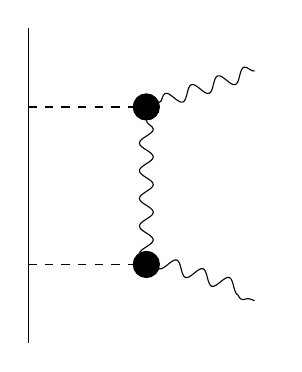
\begin{tikzpicture}

		\begin{scope}		
			\node (A1) at (3,1.5) {};
			\node (A2) at (3,-1.5){};

		\node[circle,draw,fill=black]  (V1) at (1.5,1) {}; 
		\node[circle,draw,fill=black]  (V2) at (1.5,-1) {};  
		\draw[decorate, decoration={snake}]  (V1) --  (A1);
		\draw[decorate, decoration={snake}] (V1) -- (V2) -- (A2);
		\draw[dashed](0,-1) -- (V2);
		\draw[dashed] (0,1) -- (V1);

		\draw (0,2) -- (0,-2);	
	\end{scope}
	\end{tikzpicture}
	\label{fig:orderN}
	\caption{The order $N$ term.}  
\end{figure}

Our goal is to compute the anomaly associated to the diagram in Figure \ref{fig:orderN}.

The vertices of this diagram are labeled by the Lagrangian
\[
\int_{\C^{3|4}} \mu_{BR} (w,\eta_a) \mu_1(\eta_a) \mu_2(\eta_a) \, \d z \d^2 w \d^4 \eta .
\]
where the Beltrami differential encoding the backreaction satisfies the defining equation
\[
\dbar \mu_{BR} (w,\eta_a) = \delta_{w_i=0} F^{ab} \eta_a \eta_b \partial_z  .
\]

The weight of the diagram in Figure \ref{fig:orderN} is 
\beqn
\int_{(z,w,\eta), (z',w', \eta')} \mu_{BR} (w,\eta) \mu_{w_i}(z,w,\eta) P(z , w, \eta ; z', w', \eta) \mu_{BR}(w',\eta') \mu_{w_j}(z',w',\eta') .
\eeqn
We observe that this weight is only nonzero when the inputs $\mu_{w_i}, \mu_{w_j}$ have no $\eta$-dependence.
Write $\mu_{w_i}(z,w) = \mu_{w_i}(z,w,\eta=0)$. 
Then, the diagram simplifies to 
\beqn
N \int_{(z,w), (z',w')} \mu_{BR} (w) \mu_{w_i}(z,w) \til P(z , w ; z', w') \mu_{BR}(w') \mu_{w_j}(z',w') 
\eeqn
where $\til P$ is the propagator for Kodaira--Spencer theory on $\C^3$ and $\mu_{BR}(w)$ is the distributional Beltrami differential which satisfies $\dbar \mu_{BR} (w) = \delta_{w=0} \del_z$.
We have used the notation $N = \int_{\C^{0|4}} F^2$ where $F = F^{ab} \eta_a \eta_b$. 

We compute the gauge anomaly for this diagram. 
There are two types of terms, the first is
\beqn\label{loop1}
N \int_{(z,w), (z',w')} \mu_{BR} (w) \dbar \fc_{i}(z,w) \til P(z , w ; z', w') \mu_{BR}(w') \mu_{j}(z',w') 
\eeqn
and the second is 
\beqn\label{loop2}
N \int_{(z,w), (z',w')} \mu_{BR} (w) \dbar \mu_{i}(z,w) \til P(z , w ; z', w') \mu_{BR}(w') \dbar \fc_{j}(z',w') 
\eeqn

Let's first consider \eqref{loop1}.
If we apply integration by parts to the operator $\dbar$, we see that this integal can be written as  
\begin{multline}
N \int_{(z,w), (z',w')} \dbar \mu_{BR} (w) \fc_{i}(z,w) \til P(z , w ; z', w') \mu_{BR}(w') \mu_{j}(z',w') \\
+ N \int_{(z,w), (z',w')} \mu_{BR} (w) \fc_{i}(z,w) \dbar \til P(z , w ; z', w') \mu_{BR}(w') \mu_{j}(z',w') .
\end{multline}

\subsection{The order $N^{1/2}$ term}


\section{Superconformal algebra}

\begin{itemize}
\item The bosonic operator $T = T^0 [0,0]|_{\eta = 0}$ is the stress energy tensor in the superconformal algebra. 
\item The bosonic operators $J [r,s]|_{\eta = 0}$, for $r + s = 2$ comprise the $SU(2)_R$ current.
Denote $J_0 = J [1,1]|_{\eta = 0}$, $J_+ = J^0 [2,0]|_{\eta = 0}$, $J_- = J^0[0,2]|_{\eta = 0}$. 
\item The fermionic elements of the superconformal algebra are given by the pair of $SU(2)_R$ doublets 
\[
\begin{pmatrix} G_+ \\ \Bar{G}_+ \end{pmatrix} = \begin{pmatrix} \sqrt{2} G^0_\alpha [1,0]|_{\eta = 0} \\ \sqrt{2} G^0_\gamma [1,0]|_{\eta = 0} \end{pmatrix} , \quad \begin{pmatrix} G_- \\ \Bar{G}_- \end{pmatrix} = \begin{pmatrix} \sqrt{2} G^0_\alpha [0,1]|_{\eta = 0} \\ \sqrt{2} G^0_\gamma [0,1]|_{\eta = 0} \end{pmatrix}
\]
\end{itemize}


\subsection{The $TT$ OPE}

In Section \ref{sec:TT1} we computed the tree-level $TT$ OPE at the level of general $w$-descendants.
Specializing just to $T (z) = T^0[0,0](z)$ we find that the tree-level OPE becomes the usual charge zero Virasoro OPE
\[
T(0) T(z) \simeq 2 \frac{1}{z^2} T(0) + \frac{1}{z} \partial_z T(0) .
\]

At the quantum level, this OPE is deformed. 
In \S \ref{sec:oneloop} we have shown that there is a one-loop correction to the $\til J \til J$ OPE of the form 
\[
\til J^{1}[1,0] (0, \what\eta = 0) \til J^{2} [0,1] (z, \what\eta'=0) |_{\text{1-loop}} \simeq \frac{N^2}{z^2} .
\]
Now, since 
\[
T[0,0] (\eta) = \til T[0,0] (\eta) - \frac12 \left(\del_z \til J^{1}[1,0] (\eta) - \del_z \til J^{2}[0,1] (\eta) \right) 
\]
we see that 
\[
T(0) T(z)|_{\text{1-loop}} \simeq \# \del_z^2 \frac{N^2}{z^2} = \# \frac{N^2}{z^4} .
\]

Here, we note that for type reasons, there is no one-loop quantum correction to the $\til T \til T$ OPE so that the the tree-level plus one-loop $TT$ OPE reads
\[
T(0) T(z) \simeq \# \frac{N^2}{z^4} + 2 \frac{1}{z^2} T(0) + \frac{1}{z} \partial_z T(0) .
\]


\subsection{The $JJ$ OPE } 

From \eqref{eqn:TJtree} and we see that the $SU(2)$ currents $J_0, J_\pm$ are weight one primary operators
\[
T(0) J_\pm (z) \simeq \frac1z \partial_z J_\pm (0) + \frac{1}{z^2} J_\pm (0) 
\]
and similarly for $J_0$. 


\end{document}
